\chapter{Kravspecifikation}
\section{Aktør-kontekstdiagram}

\begin{figure}[h]
\centering
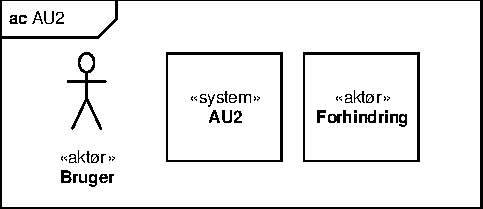
\includegraphics[width=\textwidth - 3 cm]{../fig/diagrammer/ac_au2.pdf}
\caption{Aktør kontekst diagram for AU2.}
\label{fig:aktor_kontekst}
\end{figure}

\section{Aktørbeskrivelser}
\subsubsection{Bruger - Primær Aktør}
Bruger kan:
\begin{itemize}
\item Starte og stoppe systemet 
\item Styre bilen over et netværk.
\item Deaktivere og aktivere anti-kollisionssystem.
\item (Vælge forskellige grader af anti-kollisionssystem??)
% Der menes her, at det skal være muligt at vælge imellem bremse- og styreting skal være aktivt eller ej.
\end{itemize}

\section{Funktionelle krav}
Systemet\ldots
\begin{enumerate}\itemsep1pt \parskip0pt \parsep0pt
	\item \ldots  \emph{Skal} kunne køre frem og tilbage.
	\item \ldots  \emph{Skal} kunne dreje.
	\item \ldots  \emph{Skal} kunne regulere hastigheden på bilen.
	\item \ldots  \emph{Skal} give Bruger mulighed for at begrænse maksimumshastighed.
	\item \ldots  \emph{Skal} give Bruger mulighed for manuel styring af hastighed og retning.
	\item \ldots  \emph{Skal} via Wi-Fi kunne kommunikere mellem bil og computer.
	\item \ldots  \emph{Skal} kunne identificere forhindringer foran og bag bilen.
	\item \ldots  \emph{Skal} indholde et anti-kollisionssystem baseret på afstandssensorer.
	\item \ldots  \emph{Skal} via. anti-kollisionssystemet kunne undvige og/eller stoppe før kollision.
	\item \ldots  \emph{Skal} indeholde et kamera til at streame video.
	\item \ldots  \emph{Bør} give Bruger mulighed for at aktivere/deaktivere anti-kollisionssystemet på bilen.
	\item \ldots  \emph{Kan} indeholde en batteriniveau-indikator.
\end{enumerate}

\section{Ikke-funktionelle krav}
\begin{enumerate}
	\item Bilens maksimumshastighed uden begrænsning er 20km/t $\pm$ 5\% %TODO Passer denne?
	\item Bilens bremselængde ved maksimumshastighed uden begrænsning må ikke overstige 1 m. %TODO Passer denne?
	\item Bilen skal kunne accelerere fra 0 km/t til maksimumshastighed uden begrænsning på højest 6 s. %TODO Passer denne?
	\item Forsinkelse fra brugerinput til at bilen reagerer må ikke overstige 50ms. %TODO Passer denne?
	\item Afstandssensorerne skal kunne identificere en forhindring på mindst $(30cm \times 30cm)$ på en maksimal afstand af 6 m. %TODO Passer denne, EMC - spørg vejleder?
	\item Mister bilen forbindelsen med computeren i mere end 50ms, standser bilen automatisk. 
	\item Kameraet skal minimum have en opdateringshastighed på 15 billeder i sekundet. %TODO undersøg!
	\item Systemet skal vise video-feed med en opløsning på $640 \times 480$ pixels.
	\item Computeren skal som minimum sende kommandoer til bilen 60 gange i sekundet. 
	\item HID skal bestå af en XBOX360 controller og tastatur.
\end{enumerate}

\newpage
\section{Use Cases}



% UC1:  Aktiver system
\newpage
\subsection{Use Case 1: Aktiver system}
\begin{longtable}{| l | >{\raggedright}X | >{\raggedright}X | >{\raggedright}X | >{\raggedright\arraybackslash}p{2.3cm} |} \hline
	\multicolumn{2}{|l|}{\textbf{Use case under test}} & 
	\multicolumn{3}{l|}{UC1: Aktiver system} \\ \hline
	
	\multicolumn{2}{|l|}{\textbf{Scenarie}} & 
	\multicolumn{3}{l|}{Hovedscenarie} \\ \hline
	
	\multicolumn{2}{|l|}{\textbf{Forudsætning}} & 
	\multicolumn{3}{p{10.2cm}|}{Netværksforbindelse er opsat og fungerende\hfill} \\ \hline
	%\multicolumn{5}{|l|}{}\\ \hline
	\textbf{Step} & \textbf{Handling} & \textbf{Forventet Resultat} & \textbf{Resultat} & \textbf{Godkendt / Kommentar} \\ \hline

	1.1 & Bruger sætter bilens ''ON/OFF''-switch til ''ON''. 
		& Visuel test:\\ Lampe på bilens strømforsyning lyser.
		& Lampen lyser ikke, strømforsyning kan høres. Pi og PSoC starter op og deres respektive LEDer lyser.
		& IKKE OK - Forsyning til lampe på strømforsyningen er ikke forbundet.\\ \hline
		
	1.2 & Bruger starter software på PC.
		& Visuel test:\\ Hovedvinduet vises på skærmen.
		& Hovedvinduet ses på skærmen
		& OK\\ \hline
		
	1.3 & Bruger trykker på ''Opret forbindelse''.
		& Visuel test:\\ Hovedvindue viser ''Forbindelse oprettet''.
		& En pop-op med forbindelse oprettet vises
		& OK\\ \hline
		
	1.4 & Bruger observerer hovedvinduet.
		& Visuel test:\\ Videostream vises i hovedvinduet.
		& Videostream kan ses i hovedvinduet
		& OK\\ \hline
		
	1.5 & Bruger observerer hovedvinduet.
		& Visuel test:\\ Bilens aktuelle hastighed vises i hovedvinduet.
		& Bilens hastighed vises i hovedvinduet, opdateres dog ikke hvis bilen står stille (viser ej 0 km/t)
		& OK\\ \hline
		
	1.6 & Bruger observerer hovedvinduet.
		& Visuel test:\\ Bilens aktuelle tyngdeacceleration vises i hovedvinduet.
		& Acceleration G opdateres ikke
		& IKKE OK - Accelerometer er ikke implementeret.\\ \hline
		
	1.7 & Bruger observerer hovedvinduet.
		& Visuel test:\\ Data fra bilens afstandssensorer vises i hovedvinduet.
		& Hovedvinduet viser korteste afstand for sensorerne i meter - ikke præcis over 1m
		& OK\\ \hline
		
\caption{Accepttest for UC1: Aktiver system}\label{tbl:acceptuc1}
\end{longtable}

% UC2: Stream Videofeed
\newpage
\subsection{Use Case 2: Stream Video}
\begin{longtable}{| l | >{\raggedright}X | >{\raggedright}X | >{\raggedright}X | >{\raggedright\arraybackslash}p{2.3cm} |} \hline
	\multicolumn{2}{|l|}{\textbf{Use case under test}} & 
	\multicolumn{3}{l|}{UC2: Stream Video} \\ \hline
	
	\multicolumn{2}{|l|}{\textbf{Scenarie}} & 
	\multicolumn{3}{l|}{Hovedscenarie} \\ \hline
	
	\multicolumn{2}{|l|}{\textbf{Forudsætning}} & 
	\multicolumn{3}{p{10.2cm}|}{UC1 frem til punkt 5 er fuldført \hfill} \\ \hline
	%\multicolumn{5}{|l|}{}\\ \hline
	\textbf{Step} & \textbf{Handling} & \textbf{Forventet Resultat} & \textbf{Resultat} & \textbf{Godkendt / Kommentar} \\ \hline

	2.1 & Bruger åbner AU2 softwaren på PC'en og trykker ''Opret forbindelse''. %TODO: Dobbelttjek navngivning her.
		& Visuel test:\\ Der vises et live-feed fra bilens kamera.
		& Videostream kan ses i hovedvinduet.
		& OK\\ \hline
	2.2 & Bruger har Wireshark åbent på samme computer. Wireshark er opsat til at overvåge det pågældene netværk.
		& Visuel test:\\ I Wireshark observeres der for overføring af pakker fra bilens IP-adresse til computerens IP-adresse.
		& Der overføres pakker fra Pi til computeren.
		& OK\\ \hline
		
\caption{Accepttest for UC2: Stream Video}\label{tbl:acceptuc2}
\end{longtable}

% UC3: Overvåg sensor
\newpage
\subsection{Use Case 3: Overvåg sensor}
\subsubsection{Use Case 3: Overvåg sensor}

%-------------------- UC3 --------------------
\begin{table}[h]
\begin{tabularx}{\textwidth}{| >{\raggedright\arraybackslash}p{3.3 cm} | >{\raggedright\arraybackslash}X |} \hline

\textbf{Navn:} 						 & UC3: Overvåg sensorer				\\ \hline
\textbf{Mål:}						 & At overvåge sensorer 				\\ \hline
\textbf{Initiering:}				 & UC1: Aktiver system 					\\ \hline
\textbf{Aktører:} 					 & Ingen 								\\ \hline
\textbf{Reference:} 				 & UC1, UC4: Undvig forhindring,UC9: Tænd/sluk AKS	\\ \hline
\textbf{Antal samtidige forekomster:}& Én 									\\ \hline
\textbf{Forudsætning:} 				 & UC1 frem til punkt 7 er fuldført		\\ \hline
\textbf{Resultat:}					 & Sensorer overvåges løbende  			\\ \hline
\textbf{Hovedscenarie:}				 & 

\begin{packed_enum}
	\item Bilen initierer tachometer
		\begin{packed_item}\itemsep1pt \parskip0pt \parsep0pt
			\item {[}Ext 1.a: Initiering af tachometer fejler{]}
		\end{packed_item}
	\item Bilen initierer accelerometer
		\begin{packed_item}\itemsep1pt \parskip0pt \parsep0pt
			\item {[}Ext 2.a: Initiering af accelerometer fejler{]}
		\end{packed_item}
	\item Bilen initierer afstandssensorer.
		\begin{packed_item}\itemsep1pt \parskip0pt \parsep0pt
			\item {[}Ext 3.a: Initiering af afstandssensorer fejler{]}
		\end{packed_item}
	\item Bilen overvåger sensorer.
	\item UC4: Undvig forhindring initieres af System
	\begin{packed_item}\itemsep1pt \parskip0pt \parsep0pt
			\item {[}Ext 5.a: AKS er slukket via UC9: Tænd/sluk AKS{]}
		\end{packed_item}
	\item Bilen modtager data fra PC.
	\item Bilen sender sensor data til PC.
\end{packed_enum} 															\\ \hline

\textbf{Udvidelser:}				&  
\textbf{{[}Ext 1.a : Initiering af tachometer fejler{]}}
	\begin{packed_enum}\itemsep1pt \parskip0pt \parsep0pt
		\item Systemet prompter PC med ''tachometer-initiering fejlet''.
		\item UC2 afsluttes.
	\end{packed_enum}	
														
\textbf{{[}Ext 2.a : Initiering af accelerometer fejler{]}}
	\begin{packed_enum}\itemsep1pt \parskip0pt \parsep0pt
		\item Systemet prompter PC med ''accelerometer-initiering fejlet''.
		\item UC2 afsluttes.
	\end{packed_enum}
	
\textbf{{[}Ext 3.a : Initiering af afstandssensorer fejler{]}}
	\begin{packed_enum}\itemsep1pt \parskip0pt \parsep0pt
		\item Systemet prompter PC med ''afstandssensor-initiering fejlet''.
		\item UC2 afsluttes.
	\end{packed_enum}
	
	\textbf{{[}Ext 5.a : AKS er slukket via UC9: Tænd/sluk AKS{]}}
	\begin{packed_enum}\itemsep1pt \parskip0pt \parsep0pt
		\item Use casen fortsætter fra punkt 6.
	\end{packed_enum}														\\\hline

\end{tabularx}
\caption{UC3: Overvåg sensorer}
\label{tbl:UC3}
\end{table}

% UC4: Aktiver AKS
\newpage
\subsection{Use Case 4: Aktiver AKS}

\begin{longtable}{| l | >{\raggedright}X | >{\raggedright}X | >{\raggedright}X | >{\raggedright\arraybackslash}p{2.3cm} |} \hline
	\multicolumn{2}{|l|}{\textbf{Use case under test}} & \multicolumn{3}{l|}{UC4: Undvig forhindring} \\ \hline
	\multicolumn{2}{|l|}{\textbf{Scenarie}} & \multicolumn{3}{l|}{Hovedscenarie} \\ \hline
	\multicolumn{2}{|l|}{\textbf{Forudsætning}} & \multicolumn{3}{p{10.2cm}|}{UC1 er gennemført, UC3 er gennemført.\hfill} \\ \hline
	%\multicolumn{5}{|l|}{}\\ \hline
	\textbf{Step} & \textbf{Handling} & \textbf{Forventet Resultat} & \textbf{Resultat} & \textbf{Godkendt / Kommentar} \\ \hline
	
	4.1 & Bruger styrer bilen fremad mod en forhindring på min. $(30cm \times 30cm)$ vinkelret på bilens kørebane vha. Xbox-360 controlleren, således at bilen er umiddelbart til venstre for objektet. & Visuel test: \\ Bruger observerer at bilen ændrer kurs til højre på trods af brugerinput. & ~ & ~ \\ \hline
	
	4.2 & Bruger tester om det er muligt at styre bilen igen med Xbox-360 controlleren. & Visuel test: \\ Bruger observerer at bilen reagerer på brugerinput. & ~  & ~ \\ \hline
	
	4.3 & Bruger styrer bilen fremad mod en forhindring på $(30cm \times 30cm)$ vinkelret på bilens kørebane vha. Xbox-360 controlleren, således at bilen er umiddelbart til højre for objektet. & Visuel test: \\ Bruger observerer at bilen ændrer kurs til venstre på trods af brugerinput. & ~ & ~\\ \hline
	
	4.4 & Bruger styrer bilen fremad mod en forhindring på $(30cm \times 30cm)$ vinkelret på bilens kørebane vha. Xbox-360 controlleren, således at bilen har retning lige mod objektet. & Visuel test: \\ Bruger observerer at bilen standser på trods af brugerinput. & ~ & ~ \\\hline
	
	4.5 & Bruger bakker mod en forhindring på $(30cm \times 30cm)$ vinkelret på bilens kørebane vha. Xbox-360 controlleren, således at bilen er umiddelbart til venstre for objektet. & Visuel test: \\ Bruger observerer at bilen ændrer kurs til venstre på trods af brugerinput. & ~ & ~ \\ \hline
	
	4.6 & Bruger bakker bilen mod en forhindring på $(30cm \times 30cm)$ vinkelret på bilens kørebane vha. Xbox-360 controlleren, således at bilen er umiddelbart til højre for objektet. & Visuel test: \\ Bruger observerer at bilen ændrer kurs til højre på trods af brugerinput. & ~ & ~\\ \hline
	
	4.7 & Bruger bakker bilen mod en forhindring på $(30cm \times 30cm)$ vinkelret på bilens kørebane vha. Xbox-360 controlleren, således at bilen har retning lige mod objektet. & Visuel test: \\ Bruger observerer at bilen standser på trods af brugerinput. & ~ & ~\\\hline

\caption{Accepttest for UC4: Undvig forhindring}\label{tbl:acceptuc4}
\end{longtable}

% UC5: Kør bil frem/tilbage
\newpage
\subsection{Use Case 5: Kør bil frem/tilbage}
\subsection{Use Case 5: Kør bil frem/tilbage}
\begin{table}[h]
\begin{tabularx}{\textwidth}{| L{3.3 cm} | Z |} \hline

\textbf{Navn:} 						& UC5: Kør bil frem/tilbage\\ \hline
\textbf{Mål:}						& At få bilen til at køre frem eller tilbage. \\ \hline
\textbf{Initiering:}				& Bruger \\ \hline
\textbf{Aktører:} 					& Bruger \\ \hline
\textbf{Reference:} 				& Ingen \\ \hline
\textbf{Antal samtidige forekomster:} & Én \\ \hline
\textbf{Forudsætning:} 				& UC1: Aktiver system er fuldført og systemet er operationelt. \\ \hline
\textbf{Resultat:}					& Bilens hastighed er ændret. \\ \hline
\textbf{Hovedscenarie:}				& 

\begin{packed_enum}
\item Bruger ændrer position af RT på HID controlleren.
	\begin{packed_item}\itemsep1pt \parskip0pt \parsep0pt
	\item {[}Ext 1.a: Bruger ændrer position af LT.{]}
	\end{packed_item}
\item Controllerens input streames til bilen.
\item Bilen ændrer fremadgående hastighed i henhold til brugerens input. Et hårdere tryk resulterer i en højere hastighed og et lettere tryk resulterer i en lavere hastighed.
\item UC5 afsluttes.
\end{packed_enum} \\ \hline
\textbf{Udvidelser:}				&  
\textbf{{[}Ext 1.a : Bruger ændrer position af LT.{]}}
	\begin{packed_enum}\itemsep1pt \parskip0pt \parsep0pt
		\item Controllerens input streames til bilen.
		\item Bilen ændrer bagudgående hastighed i henhold til brugerens input. Et hårdere tryk resulterer i en højere hastighed og et lettere tryk resulterer i en lavere hastighed.
		\item Systemet fortsætter fra punkt 4 i hovedscenariet.
	\end{packed_enum}
\\ \hline
\end{tabularx}
\caption{UC5: Kør bil frem/tilbage}
\label{tbl:UC5}
\end{table}

% UC6: Drej bil til højre/Venstre
\newpage
\subsection{Use Case 6: Drej bil til højre/venstre}
\subsection{Use Case 6: Drej bil til højre/venstre}
\begin{table}[h]
\begin{tabularx}{\textwidth}{| L{3.3 cm} | Z |} \hline

\textbf{Navn:} 						& UC6: Drej til højre/venstre\\ \hline
\textbf{Mål:}						& At få bilen til at dreje mod højre eller venstre. \\ \hline
\textbf{Initiering:}				& Bruger \\ \hline
\textbf{Aktører:} 					& Bruger eller AKS \\ \hline
\textbf{Reference:} 				& Ingen\\ \hline
\textbf{Antal samtidige forekomster:} & Én \\ \hline
\textbf{Forudsætning:} 				& UC1: Aktiver system er fuldført og systemet er operationelt. \\ \hline
\textbf{Resultat:}					& Retningen på bilens forhjul er ændret. \\ \hline
\textbf{Hovedscenarie:}				& 

\begin{packed_enum}
\item Bruger ændrer position på den venstre styrepind på HID controlleren.
	\begin{packed_item}\itemsep1pt \parskip0pt \parsep0pt
	\item {[}Ext 1.a: AKS er aktiveret.{]}
	\end{packed_item}
\item Controllerens input streames til bilen.
\item Bilen tjekker input, hvis den er mere mod venstre drejer hjulet mere til venstre og omvendt. %TODO dette skal lige finpudses lidt.
\item UC6 afsluttes.
\end{packed_enum} \\ \hline
\textbf{Udvidelser:}				&  
\textbf{{[}Ext 1.a : AKS er aktiveret.{]}}
	\begin{packed_enum}\itemsep1pt \parskip0pt \parsep0pt
		\item Bilen analyserer input fra UC3.
		\item Bilen drejer til højre, hvis sensor FL registrerer en forhindrer, ditto venstre og FR.
		\item Bilen undviger forhindringen. %TODO Skal eventuelt lige finpudses
		\item Systemet fortsætter fra punkt 3 i hovedscenariet.
	\end{packed_enum}
\\ \hline
\end{tabularx}
\caption{UC6: Drej til højre/venstre}
\label{tbl:UC6}
\end{table}

% UC7: Brems bil %TODO
\newpage
%\subsection{Use Case 7: Brems bil}
%\begin{longtable}{| l | >{\raggedright}X | >{\raggedright}X | >{\raggedright}X | >{\raggedright\arraybackslash}p{2.3cm} |} \hline
	\multicolumn{2}{|l|}{\textbf{Use case under test}}  & \multicolumn{3}{l|}{UC7: Brems Bil} \\ \hline
	\multicolumn{2}{|l|}{\textbf{Scenarie}} 			& \multicolumn{3}{l|}{Hovedscenarie} \\ \hline
	\multicolumn{2}{|l|}{\textbf{Forudsætning}} 		& \multicolumn{3}{p{10.2cm}|}{UC1: Aktiver system er fuldført og systemet er operationelt.\hfill} \\ \hline
	%\multicolumn{5}{|l|}{}\\ \hline
	\textbf{Step} 	& \textbf{Handling} & \textbf{Forventet Resultat} & \textbf{Resultat} & \textbf{Godkendt / Kommentar} \\ \hline
	7.1 & Bruger trykker på ''X'' knappen på Xbox-360 controlleren. 
		& Visuel test: Bruger observerer at bilens hastighed sænkes. 
		&   
		&  \\ \hline
	
\\ \hline
\caption{Accepttest for UC7: Brems Bil }\label{tbl:acceptuc7}
\end{longtable}

% UC8: Konfigurer system %TODO
\newpage
\subsection{Use Case 8: Konfigurer system}
%-------------------- UC1 --------------------
\begin{table}[h]
\begin{tabularx}{\textwidth}{| >{\raggedright\arraybackslash}p{3.3 cm} | >{\raggedright\arraybackslash}X |} \hline

\textbf{Navn:} 						& UC8.1: Konfigurer IP-adresse\\ \hline
\textbf{Mål:}						& At konfigurere bilens IP-adresse til PC'en\\ \hline
\textbf{Initering:}					& Bruger \\ \hline
\textbf{Aktører:} 					& Bruger (primær) \\ \hline
\textbf{Reference:} 					& Ingen\\ \hline
\textbf{Antal samtidige forekomster:} & Én \\ \hline
\textbf{Forudsætning:} 				& UC1: Aktiver system er udført til punkt 3, bilen og PC er på samme netværk, samt at systemet viser ''Hovedmenu'' og at systemet er operationelt\\ \hline
\textbf{Resultat:}					& IP adressen på bilen er indstillet\\ \hline
\textbf{Hovedscenarie:}				& 

\begin{packed_enum}
\item Bruger trykker på ''Konfigurer IP''.
\item Konfigurationssmenuen for IP-adressen kommer frem og der er mulighed for at indstaste en IP-adresse
\item Bruger indtaster bilens IP-adresse
\item Bruger trykker på ''Opret forbindelse'' 
\item Menuen indikerer at der er forbindelse til bilen
	\begin{packed_item}\itemsep1pt \parskip0pt \parsep0pt
	\item {[}Ext 5.a Menuen indikerer at der ikke er forbindelse til bilen{]}
	\end{packed_item}
\item Bruger trykker på "tilbage"
\item Systemet viser "Hovedmenu"
\end{packed_enum} \\ \hline
\textbf{Udvidelser:}				&  
\textbf{[}Ext 5.a Menuen indikerer at der ikke er forbindelse til bilen{]}
	\begin{packed_enum}\itemsep1pt \parskip0pt \parsep0pt
	\item Bruger gentager fra punkt 3. 
	\end{packed_enum}
\\ \hline
\end{tabularx}
\caption{UC8: Start}
\label{tbl:UC8}
\end{table}
%-------------------- UC1 --------------------
\begin{table}[h]
\begin{tabularx}{\textwidth}{| >{\raggedright\arraybackslash}p{3.3 cm} | >{\raggedright\arraybackslash}X |} \hline

\textbf{Navn:} 						& UC8.2: Tænd/sluk AKS\\ \hline
\textbf{Mål:}						& At tænde eller slukke for AKS på bilen\\ \hline
\textbf{Initering:}					& Bruger \\ \hline
\textbf{Aktører:} 					& Bruger (primær) \\ \hline
\textbf{Reference:} 					& \\ \hline
\textbf{Antal samtidige forekomster:} & Én \\ \hline
\textbf{Forudsætning:} 				& At bruger befinder sig i "Hovedmenu" og at der er oprettet forbindelse til bilen\\ \hline
\textbf{Resultat:}					&  \\ \hline
\textbf{Hovedscenarie:}				& 

\begin{packed_enum}
\item Bruger trykker på ''AKS'' 
\item Menuen for AKS kommer frem og der er mulighed for at tænde eller slukke for AKS 
\item Menuen indikerer om der er tændt eller slukket for AKS
\item Bruger trykker tænd eller sluk efter ønske
\item Bilen slukker eller tænder for AKS systemet efter brugerens ønske
\item Menuen indikerer den nye indstilling
	\begin{packed_item}\itemsep1pt \parskip0pt \parsep0pt
	\item {[}Ext 1. Der sket ingen ændring i menuen{]}
	\end{packed_item}
\end{packed_enum} \\ \hline
\textbf{Udvidelser:}				&  
\textbf{[}Ext 1. Der sker igen ændring i menuen{]}
	\begin{packed_enum}\itemsep1pt \parskip0pt \parsep0pt
	\item Bruger går til UC8.1. 
	\end{packed_enum}
\\ \hline
\end{tabularx}
\caption{UC8: Start}
\label{tbl:UC8}
\end{table}
%-------------------- UC1 --------------------
\begin{table}[h]
\begin{tabularx}{\textwidth}{| >{\raggedright\arraybackslash}p{3.3 cm} | >{\raggedright\arraybackslash}X |} \hline

\textbf{Navn:} 						& UC8.3: Indstil makshastighed\\ \hline
\textbf{Mål:}						& At konfigurere bilens makshastighed\\ \hline
\textbf{Initering:}					& Bruger \\ \hline
\textbf{Aktører:} 					& Bruger (primær) \\ \hline
\textbf{Reference:} 					& \\ \hline
\textbf{Antal samtidige forekomster:} & Én \\ \hline
\textbf{Forudsætning:} 				& At bruger befinder sig i "Hovedmenu" og at der er forbindelse til bilen\\ \hline
\textbf{Resultat:}					&  \\ \hline
\textbf{Hovedscenarie:}				& 

\begin{packed_enum}
\item Bruger trykker på ''Indstil makshastighed'' 
\item Menuen for makshastighed kommer frem og der er mulighed for at indstaste en makshastighed mellem 1 og 20km/h
\item Menuen indikerer bilens nuværende makshastighed
\item Bruger indtaster bilens nye makshastighed
\item Bruger trykker på ''Opdater'' 
\item Menuen viser den nye værdi som makshastighed
	\begin{packed_item}\itemsep1pt \parskip0pt \parsep0pt
	\item {[}Ext 1. Menuen indikerer ikke den nye makshastighed{]}
	\end{packed_item}
\end{packed_enum} \\ \hline
\textbf{Udvidelser:}				&  
\textbf{[}Ext 1. Menuen indikerer ikke den nye makshastighed{]}
	\begin{packed_enum}\itemsep1pt \parskip0pt \parsep0pt
	\item Bruger går til UC8.1 
	\end{packed_enum}
\\ \hline
\end{tabularx}
\caption{UC8: Start}
\label{tbl:UC8}
\end{table}

% UC9: Kalibrer system
\newpage
\subsection{Use Case 9: Kalibrer system}
\subsection{Use Case 9: Tænd/sluk AKS}
%-------------------- UC9 --------------------
\begin{table}[h]
\begin{tabularx}{\textwidth}{| L{3.3 cm} | Z |} \hline

\textbf{Navn:} 						& UC9: Tænd/sluk AKS \\ \hline
\textbf{Mål:}						& At tænde eller slukke for AKS på bilen \\ \hline
\textbf{Initering:}					& Bruger \\ \hline
\textbf{Aktører:} 					& Bruger (primær) \\ \hline  
\textbf{Reference:} 					& UC11: Kalibrer system\\ \hline
\textbf{Antal samtidige forekomster:} & Én \\ \hline
\textbf{Forudsætning:} 				& UC1: Aktiver system er udført, bilen og PC er på samme netværk, at systemet viser ''Hovedmenu'' samt at systemet er operationelt\\ \hline
\textbf{Resultat:}					&  \\ \hline
\textbf{Hovedscenarie:}				& 

\begin{packed_enum}
\item Bruger trykker på ''AKS'' 
\item Menuen for AKS kommer frem og der er mulighed for at tænde/slukke for AKS 
\item Menuen indikerer om der er tændt/slukket for AKS
\item Bruger trykker tænd/sluk efter ønske
\item Bilen tænder/slukker for AKS systemet efter brugerens ønske
\item Menuen indikerer nuværende status af AKS
\end{packed_enum} \\ \hline
\textbf{Udvidelser:}				&  
~
\\ \hline
\end{tabularx}
\caption{UC9: Tænd/sluk AKS}
\label{tbl:UC9}
\end{table}

% UC10: Afbryd system
\newpage 
\subsection{Use Case 10: Afbryd system}
\begin{longtable}{| l | >{\raggedright}X | >{\raggedright}X | >{\raggedright}X | >{\raggedright\arraybackslash}p{2.3cm} |} \hline
	\multicolumn{2}{|l|}{\textbf{Use case under test}}  & \multicolumn{3}{l|}{UC10: Indstil makshastighed} \\ \hline
	\multicolumn{2}{|l|}{\textbf{Scenarie}} 			& \multicolumn{3}{l|}{Hovedscenarie} \\ \hline
	\multicolumn{2}{|l|}{\textbf{Forudsætning}} 		& \multicolumn{3}{p{10.2cm}|}{UC1: Aktiver system er udført, bilen og PC er på samme netværk, at systemet viser ''Hovedvindue'' samt at systemet er operationelt.\hfill} \\ \hline
	%\multicolumn{5}{|l|}{}\\ \hline
	\textbf{Step} 	& \textbf{Handling} & \textbf{Forventet Resultat} & \textbf{Resultat} & \textbf{Godkendt / Kommentar} \\ \hline
	
	10.1 & Bruger trykker på ''Indstil makshastighed''. 
		 & Visuel test: \\ Hovedvindue viser menu med mulighed for at indtaste makshastighed fra 1-10 km/t. 
		 & Vindue med mulighed for indstilling af max hastighed vises.
		 & OK\\ \hline
	10.2 & Menuen viser bilens nuværende makshastighed. 
		 & Den nuværende makshastighed vises.
		 & Den nuværende makshastighed vises til højre.
		 & OK\\ \hline
	10.3 & Bruger indtaster bilens ønskede makshastighed. 
		 & Menuen viser den ønskede makshastighed. 
		 & Der vises den nye makshastighed 
		 & OK\\ \hline
	10.4 & Bruger trykker på ''Ok''. 
		 & Systemet viser den nye makshastighed. 
		 & Systemet viser den indstillede makshastighed
		 & OK\\ \hline
	10.5 & Bruger holder ''RT'' inde på Xbox 360 controlleren.
		 & Bilen accelerer til den angivne maksimalhastighed.
		 & Bilen ændrer makshastighed ift. den indtastede, dette er dog ikke målt præcist
		 & MÅSKE OK\\ \hline
		 
\caption{Accepttest for UC10: Indstil makshastighed }\label{tbl:acceptuc10}
\end{longtable}